\documentclass{article}
\usepackage{asymptote}
% Erin's additions
\usepackage{color} 
\usepackage{tikz}
\usepackage{youndtab}
\usetikzlibrary{decorations.pathmorphing}
\usetikzlibrary{decorations.fractals}

\begin{document}

\section{Ferrers' Diagram for a Partition}
% Define a partition $(\lambda_1 + \lambda_2 + \cdots + \lambda_k) \vdash n$.\\
% Draw $k$ lines opf dots, left justified, $\lambda_j$ dots in the $j^{\text{th}}$ line.

\begin{Young}
$a$&&\cr
&\cr
\cr
\end{Young}

\begin{center}
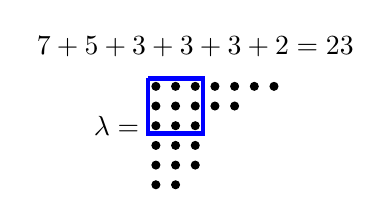
\begin{tikzpicture}
\draw (.5,.5) node {$7 + 5 + 3 + 3 + 3 + 2 = 23$};
\draw (-.5, -.5) node {$\lambda = $ };
\foreach \x in {0,...,6}
  \filldraw (\x*.25, 0) circle (.5mm);
\foreach \x in {0,...,4}
  \filldraw (\x*.25, -.25) circle (.5mm);
\foreach \x in {0,...,2}
  \filldraw (\x*.25, -.5) circle (.5mm);
\foreach \x in {0,...,2}
  \filldraw (\x*.25, -.75) circle (.5mm);
\foreach \x in {0,...,2}
  \filldraw (\x*.25, -1) circle (.5mm);
\foreach \x in {0,...,1}
  \filldraw (\x*.25, -1.25) circle (.5mm);
\draw[ultra thick, blue] (-.1,0.1) -- (-.1,-.6) -- (.6, -.6) -- (.6, .1) -- (-.1,.1);
\end{tikzpicture}
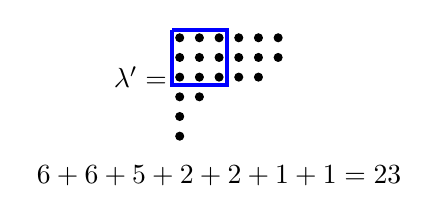
\begin{tikzpicture}
\draw (.5,-1.75) node {$6 + 6 + 5 + 2 + 2 + 1 + 1 = 23$};
\draw (-.5, -.5) node {$\lambda^\prime = $ };
\foreach \x in {0,...,5}
  \filldraw (\x*.25, 0) circle (.5mm);
\foreach \x in {0,...,5}
  \filldraw (\x*.25, -.25) circle (.5mm);
\foreach \x in {0,...,4}
  \filldraw (\x*.25, -.5) circle (.5mm);
\foreach \x in {0,...,1}
  \filldraw (\x*.25, -.75) circle (.5mm);
\filldraw (0, -1) circle (.5mm);
\filldraw (0, -1.25) circle (.5mm);
\draw[ultra thick, blue] (-.1,.1) -- (-.1,-.6) -- (.6, -.6) -- (.6, .1) -- (-.1,.1);
\end{tikzpicture}
\end{center}

\begin{figure}[!ht]
    \centering
    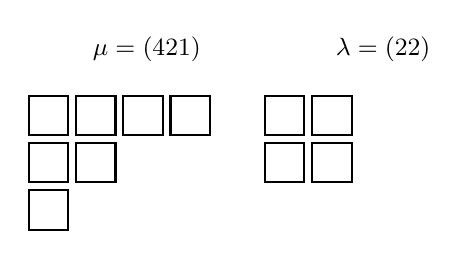
\begin{tikzpicture}[thick]
%      \draw[style=help lines] (0,0) grid (9,3);
      \foreach \position in {(0,0),(0,0.6),(0,1.2),(0.6,0.6),(0.6,1.2),(1.2,1.2),(1.8,1.2)}
        \draw \position rectangle +(0.5,0.5);
      \draw (1.5,2) node[above] {\small $\mu=(421)$};
      \begin{scope}[xshift=3cm]
        \foreach \position in {(0,0.6),(0,1.2),(0.6,0.6),(0.6,1.2)}
        \draw \position rectangle +(0.5,0.5);
        \draw (1.5,2) node[above] {\small $\lambda=(22)$};
      \end{scope}
      % \begin{scope}[xshift=6cm]
      %   \foreach \position in {(0,0),(1.2,1.2),(1.8,1.2)}
      %     \draw \position rectangle +(0.5,0.5);
      %   \draw (1.5,2) node[above] {\small \lambda};
      % \end{scope}
    \end{tikzpicture}
    % \caption[Examples of \textsc{Ferrers} diagrams]{Examples of \textsc{Ferrers} diagrams. Note that $\nicefrac{\mu}{\lambda}$ is not a border strip.}\label{fig:ferrers}
  \end{figure}




% \begin{figure}[!ht]
%     \centering
%     \begin{subfigure}{0.2\linewidth}
%       \centering
%       \begin{tikzpicture}[thick]
% %        \draw[style=help lines] (0,0) grid (3,2);
%         \foreach \position in {(0,0),(0,0.6),(0,1.2),(0.6,0.6),(0.6,1.2),(1.2,1.2),(1.8,1.2)}
%         \draw \position rectangle +(0.5,0.5);
%       \end{tikzpicture}
%       \caption{$\mu=(421)$}\label{subfig-1:ferrers}
%     \end{subfigure}
%     \begin{subfigure}{0.2\linewidth}
%       \centering
%       \begin{tikzpicture}[thick]
% %        \draw[style=help lines] (0,0) grid (3,2);
%         \foreach \position in {(0,0.6),(0,1.2),(0.6,0.6),(0.6,1.2)}
%         \draw \position rectangle +(0.5,0.5);
%         \foreach \position in {(0,0),(1.2,1.2),(1.8,1.2)}
%         \path \position rectangle +(0.5,0.5);
%       \end{tikzpicture}
%       \caption{$\lambda=(22)$}\label{subfig-2:ferrers}
%     \end{subfigure}
%     \begin{subfigure}{0.2\linewidth}
%       \centering
%       \begin{tikzpicture}[thick]
% %        \draw[style=help lines] (0,0) grid (3,2);
%         \foreach \position in {(0,0),(1.2,1.2),(1.8,1.2)}
%         \draw \position rectangle +(0.5,0.5);
%         \foreach \position in {(0,0.6),(0,1.2),(0.6,0.6),(0.6,1.2)}
%         \path \position rectangle +(0.5,0.5);
%       \end{tikzpicture}
%       \caption{$\nicefrac{\mu}{\lambda}$}\label{subfig-3:ferrers}
%     \end{subfigure}
%     \caption[Examples of \textsc{Ferrers} diagrams]{Examples of \textsc{Ferrers} diagrams. Note that $\nicefrac{\mu}{\lambda}$ is not a border strip.}\label{fig:ferrers}
% \end{figure}

% \begin{figure}
% \centering
% \begin{asy}
% unitsize(6mm);
% struct Ferrer {
%         static path Box = box((0, 0), (0.8, -0.8));
%         static int offset = 0;
%         bool[][] values;
%         bool get(int i, int j) {
%                 return values.initialized(i) && values[i].initialized(j) && values[i][j];
%         }
%         void set(int i, int j) {
%                 if(!values.initialized(i)) values[i] = new bool[];
%                 values[i][j] = true;
%         }
%         void operator init(...int[] r) {
%                 for(int i = 0; i < r.length; ++i) {
%                         for(int j = 0; j < r[i]; ++j) set(i,j);
%                 }
%         }
%         void Draw(string L) {
%                 int n = 0;
%                 for(int i = 0; i < values.length; ++i) {
%                         n = max(n, values[i].length);
%                         for(int j = 0; j < values[i].length; ++j) {
%                                 currentpen = get(i,j) ? defaultpen : nullpen;
%                                 draw(shift(offset+j, -i) * Box);
%                         }
%                 }
%                 label(L, (offset+n/2, 0), N, defaultpen);
%                 offset += n+2;
%         }
% }
% Ferrer operator/(Ferrer L, Ferrer R) {
%         Ferrer result;
%         for(int i = 0; i < L.values.length; ++i) {
%                 for(int j = 0; j < L.values[i].length; ++j) {
%                         if(L.get(i,j) && !R.get(i,j)) result.set(i,j);
%                 }
%         }
%         return result;
% }
% Ferrer mu = Ferrer(4, 2, 1);
% Ferrer lambda = Ferrer(2, 2);
% mu.Draw("$\mu = (421)$");
% lambda.Draw("$\lambda = (22)$");
% (mu/lambda).Draw("$\mu/\lambda$");
% \end{asy}
% \caption{Examples of \textsc{Ferrers} diagrams. Note that $\mu/\lambda$ is not a border strip.}
% \end{figure}


\end{document}